\documentclass{report}


\usepackage[italian]{babel}

% Set page size and margins
% Replace `letterpaper' with `a4paper' for UK/EU standard size
\usepackage[letterpaper,top=2cm,bottom=2cm,left=3cm,right=3cm,marginparwidth=1.75cm]{geometry}

% Useful packages
\usepackage{amsmath}
\usepackage{float}
\usepackage{graphicx}
\usepackage[colorlinks=true, allcolors=blue]{hyperref}
\usepackage[T1]{fontenc}
\usepackage[utf8]{inputenc}
\usepackage{setspace}
\usepackage[paper=a4paper,margin=1in]{geometry}
\usepackage[square,numbers,super]{natbib}
\usepackage[nottoc]{tocbibind}


\begin{document}


\begin{titlepage}
        
        \noindent
        \begin{minipage}[t]{0.19\textwidth}
            \vspace{-4mm}{
\includegraphics[scale=1.15]{logo_unimib.pdf}}
        \end{minipage}
        \begin{minipage}[t]{0.81\textwidth}
        {
                \setstretch{1.42}
                {\textsc{Università degli Studi di Milano - Bicocca}} \\
                \textbf{Scuola di Scienze} \\
                \textbf{Dipartimento di Informatica, Sistemistica e Comunicazione} \\
                \textbf{Corso di laurea in Informatica} \\
                \par
        }
        \end{minipage}
        
	\vspace{40mm}
        
	\begin{center}
            {\LARGE{
                    \setstretch{1.2}
                    \textbf{Strategie di automatizzazione di liquidità nella finanza decentralizzata}
                    \par
            }}
        \end{center}
        
        \vspace{50mm}

        \noindent
        {\large \textbf{Relatore:} Prof. Alberto Leporati } \\
        
         \noindent
        {\large \textbf{Correlatore:} Ing. Paolo Antonio Rossi}
        
        \vspace{15mm}

        \begin{flushright}
            {\large \textbf{Relazione della prova finale di:}} \\
            \large{Christian Kobril} \\
            \large{Matricola 856448} 
        \end{flushright}
        
        \vspace{40mm}
        \begin{center}
            {\large{\bf Anno Accademico 2021-2022}}
        \end{center}

        \restoregeometry
        
    \end{titlepage}

\tableofcontents

\begin{enumerate}
\item Introduzione alla Finanza Decentralizzata
\item AMM e pool di liquidità
\item Complessità di Uniswap v3
\item Orbit, piattaforma per automatizzare e ottimizzare strategie defi
\item Utilizzo degli smart vaults
\item Moduli di Orbit: autocompound, rebalance and idle liquidity
\item Tecnologie utilizzate nello sviluppo di Orbit
\item Architettura degli smart contracts
\item Future implementazioni all'interno di Orbit
\end{enumerate}





\chapter{Introduzione}
Il tema centrale di questa tesi di laurea è la \textbf{finanza decentralizzata}.\\ In particolare, si approfondirà il ruolo che la blockchain ha in questo settore, fornendo esempi di un prodotto software concretamente sviluppato durante il mio  \textit{Project Work} svolto presso l'azienda \textit{Five Elements Labs Srl}.
\\\\Inoltre, verranno approfonditi i concetti di \textit{pool di liquidità}, \textit{automated market maker(AMM)} e \textit{strategie DeFi} su Uniswap v3.

\section{Cos'è la Finanza Decentralizzata}

Il termine \textbf{finanza decentralizzata} viene usato per classificare tutti quei servizi finanziari che avvengono direttamente tra due entità su una blockchain.

\subsection{Differenze tra Finanza Decentralizzata e Tradizionale}

Per comprendere il concetto su cui si basa la finanza decentralizzata (da ora in poi \textit{DeFi}), è bene dare un rapido sguardo alla sua controparte: la finanza tradizionale (o centralizzata).\\\\
Nella finanza centralizzata, ogni singola operazione finanziaria tra due persone (bonifici, prestiti, scambio di risorse, mutui) richiede l'interazione con soggetti di terze parti (tipicamente banche o altri enti).\\
Ciò incrementa le già prolisse tempistiche burocratiche, oltre ad aggiungere i costi dovuti al servizio fornito dagli enti che permettono l'operazione.
\\\\Invece, la finanza decentralizzata permette l'interazione tra due soggetti senza l'intermediazione di un sistema centralizzato, bensì mediante un applicativo software costruito sopra la tecnologia blockchain, rendendo le operazioni rapide, pubbliche e sicure.


\section{Caratteristiche e vantaggi della DeFi}

\subsection{Applicazioni decentralizzate}
Gli applicativi software utilizzati in DeFi vengono chiamati \textit{dApps (decentralized applications)}, ovvero particolari prodotti che interagiscono con diverse blockchain. Di tali reti noi considereremo solo quella di \textbf{Ethereum}\cite{ethereum}, nota per la sua flessibilità e accessibilità.\\\\
La blockchain di Ethereum, a differenza di reti come quella di \textbf{Bitcoin}\cite{bitcoin}, è \textbf{programmabile}; ossia è possibile costruirci sopra e distribuire dApps, rendendo la rete una sorta di gigantesco marketplace in cui trovare servizi finanziari, videogiochi, social network e diverse altre applicazioni.
\\Su tale blockchain risiedono dei particolari programmi denominati \textit{Smart Contracts}\cite{smartcontracts}, i quali si occupano di garantire sicurezza, trasparenza e irreversibilità delle operazioni avvenute sulla blockchain.\\

\subsection{Accesso alle dApps}

Il concetto di login ideato nel web2, tipicamente caratterizzato dall'inserimento di un'email e una password, viene sorpassato da una nuova autenticazione del \textbf{web3}\cite{web2_web3}: attraverso il proprio \textit{portafoglio digitale} (da ora in poi, wallet \cite{wallet}) è possibile accedere al proprio account e gestire i propri assets digitali, eventualmente mettendoli a disposizione della dApp a cui si è connessi.
\\\\I wallet presentano il vantaggio di non dover fornire nomi, indirizzi fisici, email o altre informazioni personali, garantendo la riservatezza dei propri dati; basta creare un wallet per avere immediato accesso alle piattaforme, senza registrazioni.



\subsection{Operazioni in DeFi}

Ogni operazione nella DeFi viene detta \textbf{transazione}. Una transazione è permanentemente salvata sui registri della blockchain, rendendo ogni singola operazione, associata ad un identificativo, consultabile in qualsiasi momento da qualsiasi persona.
\\Tale trasparenza viene difficilmente concessa dalle banche, ponendo la DeFi come un sistema aperto e rintracciabile.

\subsection{Flessibilità}

L'ultima caratteristica della DeFi che ritengo importante citare è ciò che più la contraddistingue dalla finanza tradizionale: la sua flessibilità.\\
In qualsiasi momento un utente può trasferire i propri assets digitali, senza dover chiedere il permesso a soggetti di terze parti, evitando costose commissioni e con un'attesa che va da pochi secondi a pochi minuti. 


\chapter{Uniswap, piattaforma di Liquidity Providing}

Avendo approfondito cosa è la DeFi, quali sono le sue caratteristiche e i principali vantaggi, ritengo necessario concentrarsi su quali sono i prodotti "dApps" che hanno messo le basi per il lavoro svolto durante il mio Project Work.

\section{Uniswap}

Innanzitutto, è bene distinguere la piattaforma Uniswap\cite{uniswap} dall'omonimo protocollo.
\\La dApp di Uniswap (conosciuta come Uniswap Interface) è una piattaforma che permette agli utenti l'interazione con il protocollo Uniswap.
\\\\Quest'ultimo è una suite di Smart Contracts, per definizione persistenti e non aggiornabili, che insieme formano un \textbf{Automated Market Maker} (da ora in poi AMM)\cite{amm}.

\section{Scambi nei mercati tradizionali}

La maggior parte dei mercati tradizionali ad accesso pubblico utilizza ciò che viene definito \textit{Order Book}\cite{order_book}, ossia un elenco degli ordini di acquisto e vendita attualmente aperti per un asset, organizzati per prezzo.
\\Sostanzialmente, un \textit{sistema di corrispondenza}\cite{matching} si occupa di abbinare gli ordini di acquisto con quelli di vendita, usando l'order book per eseguire le operazioni tra i partecipanti dello scambio.


\section{Automated Market Maker}

La rivoluzione introdotta dalla blockchain sta nella possibilità di creare nuovi tipi di scambi che abbinano algoritmicamente ordini di acquisto e vendita utilizzando gli smart contracts.
\\Tali scambi vengono detti \textit{Scambi Decentralizzati (DEX)}.
\\\\Un AMM è un protocollo DEX che si basa su un algoritmo di valutazione per prezzare gli asset mediante una formula matematica.
\\Il citato order book viene rimpiazzato con una pool di liquidità\cite{liquidity_pool}, contenente due asset, entrambi valutati l'uno rispetto all'altro.
\\Quando un asset viene scambiato per un altro, i prezzi relativi dei due asset cambiano, e viene determinato un nuovo tasso di mercato per entrambi.
In questo modo acquirenti e venditori interagiscono direttamente con la pool (e di conseguenza gli smart contracts), senza dover interagire tra di loro in modo diretto.

\subsection{Esempio pratico di AMM}

Un esempio pratico che mi ha aiutato a comprendere il funzionamento degli AMM è quello dei contadini di mele e patate.
\\Immaginiamo di essere un contadino e di avere solo patate, senza la possibilità di coltivare, e di conseguenza mangiare, nient'altro.\\ Un giorno ci viene proposto di effettuare degli scambi con un venditore di mele attraverso un messaggero, il quale decide di custodire mele e patate in un contenitore magico, in modo tale che rimangano a disposizione senza marcire (e dunque perdere di valore).
\\\\La regola fondamentale per questo scambio è una sola: \textit{il contenitore magico dovrà sempre contenere lo stesso valore di mele e patate.}
\\Tale regola è in realtà la formula alla base dell'AMM di Uniswap, conosciuta come \textbf{Constant Product Formula}: 

\[ x * y = k \]
\\dove $x$ corrisponde al numero di mele e $y$ al numero di patate nel contenitore.
\\Inizialmente il contenitore sarà perfettamente bilanciato, per esempio con 500 mele e 500 patate, entrambe prezzate ad €1 per un valore totale di €1.000.
\\\\Tuttavia, se un contadino volesse scambiare le sue patate grazie al contenitore, potrebbe ricevere in cambio meno mele rispetto alle patate inviate.
Questo perché il prezzo della mela potrebbe aumentare, e dunque per bilanciare il contenitore il prezzo delle patate dovrà di conseguenza diminuire.
\\Allo stesso modo, se un contadino volesse scambiare le proprie mele, riceverebbe più patate di quelle che avrebbe ricevuto inizialmente, considerato l'aumento del prezzo della mela rispetto alle patate.
\\\\Nella realtà dei fatti, questo contenitore magico è conosciuto come \textit{pool di liquidità}.

\section{Pool di liquidità}

È possibile vedere una pool di liquidità come uno spazio in cui i contandini (trader) possono mettere a disposizione la propria liquidità di mele e patate (criptovalute, nello specifico token ERC-20\cite{erc_20}); tali utenti vengono definiti fornitori di liquidità (\textit{liquidity providers, da ora in poi LP}).
\\\\Come ricompensa per la liquidità fornita, gli \textbf{LP} ricevono commissioni sulle operazioni che avvengono nella pool a cui partecipano. 
Tali commissioni si applicano sulle singole transazioni effettuate con la liquidità fornita da un LP, e possono variare di percentuale dal 0.01\%\ fino all'1\%\.\\\\Nel caso di Uniswap, gli LP depositano un valore equivalente di due token; per esempio, 50\% ETH e 50\% USDC nella pool ETH/USDC.


\section{Protocollo Uniswap v3}

Uniswap v3 è l'ultima versione del protocollo rilasciata da Uniswap nel maggio 2021.\\ Tale protocollo definisce le funzionalità della suite di smart contracts con cui gli utenti interagiscono, introducendo importanti novità rispetto al suo predecessore, v2.

\subsection{Posizioni}

Utilizzando l'interfaccia Uniswap, gli utenti possono connettere il loro wallet personale per mettere a disposizione un certo ammontare di liquidità all'interno di una pool.
Tale liquidità, come spiegato in precedenza, dovrà mantenere un'equa proporzione tra i due asset messi a disposizione: tale operazione viene definita come \textit{apertura di una \textbf{posizione}} (o in inglese, position minting).
\\\\Su Uniswap v3, le posizioni vengono rappresentate mediante NFT (ERC-721\cite{erc_721}), i quali certificano un determinato wallet, in questo caso chi effettua il minting, come proprietario della posizione.

\subsection{Complicazioni di Uniswap v2}

\\\\In precedenza, nella v2 di Uniswap, i LP potevano mettere a disposizione i propri asset per scambi \textbf{a qualsiasi intervallo di prezzo}.
\\\\Consideriamo che io, trader che utilizza Uniswap, voglia mettere a disposizione due miei asset chiamati token $A$ e token $B$.
Ricordando che l'intervallo di prezzo che scelgo per aprire una posizione è sempre il prezzo di $A$ rispetto al prezzo di $B$ ($A$ \textbf{su} $B$), decido di scegliere un range che copra tutti i prezzi possibili.\\
In questo modo non vi è alcuna perdita di liquidità, portando però un importante svantaggio: la maggior parte della liquidità non viene mai utilizzata negli scambi.
\\\\Provando a considerare una pool contenente una coppia di due stable coins, ossia token il cui prezzo rimane relativamente costante nel tempo, possiamo assumere che la liquidità al di fuori del tipico intervallo di prezzo dei suddetti stable coins non verrebbe mai toccata.
\\\\Per esempio in Uniswap v2 la coppia DAI/USDC (\textbf{entrambi stable coins dal valore di circa \$\01}) utilizza circa il 0.50\%\ del capitale totale disponibile per gli scambi all'interno del range tra \$\00.99 e \$\11.01\cite{v2_waste}. Il resto della liquidità è distribuito nella restante fascia di prezzo tra 0 e $\infty$ (escluso il range sopra citato), rendendo quel capitale inutilizzabile (e dunque, non consentendo agli LP di guadagnare commissioni). 
\\\\Ciò è dovuto al fatto che la liquidità sia uniformemente distribuita in un range di prezzo da 0 a $\infty$, senza che sia \textit{concentrata} nel giusto intervallo: per tale ragione è stato introdotto \textbf{Uniswap v3}.

\subsection{Liquidità concentrata}
\\\\Ciò che rende Uniswap v3 un protocollo davvero valido è l'idea della \textit{Liquidità Concentrata}\cite{concentrated_liquidity}. Tale liquidità viene distribuita in un intervallo di prezzo personalizzabile, a scelta dell'utente.
\\\\Riprendendo l'esempio sopra citato, un trader potrebbe decidere di investire nella pool DAI/USDC, scegliendo come range il più proficuo, ossia quello compreso tra \$\00.99 e \$\11.01.
In tal modo, la liquidità concentrata garantirà un guadagno superiori di commissioni (da ora in poi fees) sfruttando il capitale messo a disposizione dai LPs.

\subsection{Tick di prezzo}

Per rendere la liquidità concentrata funzionale, lo spazio continuo del prezzo è stato partizionato in \textbf{tick}.
\\\\I tick sono i limiti di aree discrete nello spazio del prezzo. Tali limiti sono posizionati in modo tale che il diminuire o aumentare di 1 tick rappresenti l'aumento o la diminuzione percentuale del 0.01\%\ del prezzo in ogni punto dello spazio.
\\Dunque quando una posizione viene creata, un LP non può scegliere qualsiasi valore per il range di prezzo: è necessario che il limite inferiore (\textbf{lower tick}) e il limite superiore (\textbf{upper tick}) corrispondano a dei tick di prezzo validi.

\subsection{Swap e Fees}

Il modo più utilizzato per interagire con Uniswap v3 è tramite gli scambi (da ora in poi \textbf{swap}).
Uno swap è relativamente semplice: un utente seleziona un token ERC-20 del quale è proprietario e un token che vorrebbe scambiare per esso. Uniswap venderà il token attualmente in possesso dell'utente, restituendo una quantità proporzionale del token desiderato, sottraendo una \textbf{swap fee}, ossia quella percentuale riconosciuta ai LPs per aver messo a disposizione la loro liquidità con la quale è avvenuto lo scambio.
\\\\Tuttavia, la transazione potrebbe richiedere alcuni minuti, a seconda della rete su cui avviene, rilevando un fenomeno conosciuto come \textbf{slippage}.
\\Lo slippage è l'alterazione di prezzo di un token che avviene mentre la transazione è in attesa di essere completata. Tale alterazione ha una soglia di tolleranza dell'1\%\: superata tale soglia l'operazione viene rifiutata e lo swap annullato, onde evitare grosse perdite per l'utente.

\section{Complicazioni di Uniswap v3}

Qualora il prezzo di un token dovesse muoversi verso una direzione (di discesa o di salita), il proprietario della posizione si ritroverebbe con un ammontare superiore di uno dei due token rispetto all'altro, in quanto il prezzo dell'uno sull'altro cambierà, fino a quando l'intera liquidità sarà relativa a solo uno dei due asset.
\\\\Per esempio, se in una pool ETH/USDC il prezzo di ETH dovesse diminuire, la percentuale di liquidità relativa a ETH aumenterebbe, per bilanciare il valore immesso all'interno della posizione stessa.
Allo stesso modo, se ETH dovesse aumentare di valore, la percentuale di USDC aumenterebbe a sua volta.
\\\\Con l'aumentare o il diminuire del prezzo di un asset nella pool, tale prezzo potrebbe uscire dall'intervallo che un LP ha impostato per una certa posizione. Nel momento in cui una posizione si dovesse trovare fuori dall'intervallo scelto (\textbf{Out Of Range position}) la liquidità diventerebbe inattiva (\textbf{idle liquidity}) e l'utente proprietario di tale liquidità non guadagnerebbe più fees.
\\Tuttavia, nel momento in cui il valore del primo token sul secondo dovesse tornare nell'intervallo di prezzo iniziale, il LP tornerebbe a guadagnare fee.
\\\\È proprio dal problema della liquidità inattiva che nasce \textbf{Orbit DeFi}, il prodotto sviluppato durante il mio project work.







\chapter{Orbit, piattaforma per automatizzare strategie DeFi}

Ho avuto l'opportunità di svolgere il mio Project Work per Five Elements Labs, azienda specializzata nella produzione di software nel mondo blockchain; in particolare nei settori DeFi e NFT.
\\Durante tale esperienza, mi sono unito allo sviluppo del loro principale prodotto: \textbf{Orbit}\cite{orbit_website}.

\section{Introduzione ad Orbit}


\textbf{Orbit} è una piattaforma di gestione di liquidità nel settore DeFi: ossia un \textbf{layer} che permetta ai propri utenti di automatizzare strategie e di ottimizzare posizioni di liquidità su Uniswap v3.
\\Può essere interpretato come \textbf{un'estensione} del proprio wallet, in grado di gestire gli assets degli utenti per fornire la possibilità di ottenere un ritorno aggiuntivo dalla liquidità concentrata.

\section{Perché nasce Orbit}

Con il rapido crescere del settore DeFi e del corrispondente ecosistema di protocolli, ognuno con le proprie caratteristiche e logiche, risulta sempre più complesso gestire delle strategie di liquidità al passo con i tempi.

\subsection{Gas fee}
\\Ogni transazione avvenuta sulla blockchain ha un \textit{"costo"} chiamato \textbf{gas fee}\cite{gas}.
\\È possibile affermare che il gas sta alla blockchain come la \textbf{benzina} sta alla macchina; è necessario per far funzionare i nodi che compongono la rete.
\\Sostanzialmente è l'unità di misura dello \textit{sforzo computazionale} fatto dai nodi per sostenere una transazione, la quale può prevedere diverse complesse operazioni al suo interno.
\\Tale benzina deve essere in qualche modo pagata, per questo esistono commissioni sul gas (gas fee).
\\\\Diverse blockchain con basse gas fee (come \textbf{Polygon}\cite{polygon}) stanno diventando sempre più popolari, spostando l'attenzione degli sviluppatori e degli utenti verso la possibilità di costruire piattaforme e strumenti veloci ed efficaci.
\\\\Orbit dunque cavalca quest'onda di innovazione e di creatività, portando la liquidità concentrata verso un nuovo livello, costruendo uno strumento efficiente e facile da utilizzare per professionisti e novizi del mondo DeFi.\\\\

\section{Vantaggi per gli utenti}

Automatizzare strategie riguardo posizioni su Uniswap v3 ha un diretto impatto sui \textbf{ritorni generati} da queste ultime.
\\La maggior parte dei protocolli presenti sul mercato forniscono ai trader \textbf{strategie attive}, sulle quali è necessario compiere delle complesse scelte conosciute perlopiù da utenti professionisti.
\\\\Le funzionalità fornite da Orbit permettono agli utenti di creare \textbf{strategie passive}, senza il necessario bisogno di rimanere aggiornati sui protocolli, bensì lasciando alla piattaforma il compito di gestire la propria liquidità.
\\Inoltre, nella prima versione del protocollo, sarà Orbit ad occuparsi dei costi di gas dovuti alle transazioni rivolte agli smart contract dell'applicazione.

\section{Modelli di gestione di liquidità}

Nello stato attuale della DeFi, vi sono concretamente due modelli ben distinti di gestione di liquidità:  \textbf{Aggregatori}\cite{aggregator} e  \textbf{Smart Vaults}\cite{smart_vault}.

\subsection{Aggregatori}

Gli Aggregatori sono delle particolari piattaforme DeFi, le quali permettono ai propri utenti di effettuare transazioni verso diverse dApps \textbf{in un unico posto}. Ciò permette di risparmiare tempo e aumentare l'efficienza delle transazioni.
\\\\Tali Aggregatori permettono ai trader di \textbf{replicare} strategie di utenti esperti e di applicarle al proprio portfolio. Per esempio, possono confrontare i prezzi degli assets su diverse piattaforme, proponendo lo scambio più conveniente all'utente.
\\\\Tuttavia, protocolli utilizzatori di Aggregatori come \textit{Yearn Finance}, \textit{Beefy} o \textit{Idle} consentono all'utente l'utilizzo di strategie singole, tipicamente con un modello "\textit{Black Box}", ovvero senza verificarne l'effettivo funzionamento interno.

\subsection{Smarts vaults}

Contrariamente agli Aggregatori, gli \textbf{Smart Vaults} garantiscono un'alta \textbf{personalizzazione} delle strategie scelta direttamente dagli utenti.
\\Il funzionamento è relativamente semplice: un utente diventa \textit{proprietario} di un particolare Smart Contract effettuando una transazione che ne crea un'istanza contenente l'indirizzo del suo creatore.\footnote{Approfondimenti tecnici riguardanti la creazione dello Smart Vault e dei relativi Smart Contracts verranno trattati nel capitolo 5}.
\\Successivamente, il contratto creato viene utilizzato come \textit{un'estensione} del proprio wallet per gestire assets e per interagire con altri protocolli per consentire allocazioni automatiche di liquidità: tale Smart Contract è chiamato Smart Vault.
\\\\Il modello a Smart Vault è stato poco utilizzato in passato, principalmente a causa delle alte gas fee richieste dalle reti per attivare strategie multiple.
\\Tuttavia, con l'avvento di blockchain sempre meno costose in termini di gas, è ora possibile utilizzare gli Smart Vaults per integrare facilmente nuovi protocolli e fornire all'utente la possibilità di avere un totale controllo sulle interazioni con essi.
\\\\Per tali ragioni, il modello a Smart Vault è stato scelto per la realizzazione di Orbit.


\chapter{Tecnologie utilizzate nello sviluppo di Orbit}

Orbit è una piattaforma che prende forma nel mondo del Web3, pertanto per la sua realizzazione sono state richieste tecnologie specifiche di questo emergente settore.
\\Possiamo logicamente suddividere Orbit in due macro parti: il \textbf{frontend}, ossia l'interfaccia della dApp\cite{orbit_website} con la quale l'utente interagisce direttamente, ed il \textbf{backend} composto da una suite di contratti che racchiudono le logiche e meccanismi su cui Orbit si basa.

\section{Tecnologie Frontend e librerie utilizzate}

La scelta del linguaggio utilizzato per la dApp Orbit, trattandosi di un'applicazione web, è ricaduta sul linguaggio \textbf{Javascript}\cite{js}.\\Le caratteristiche del linguaggio, quali \textit{versatilità, leggerezza e facilità d'apprendimento} hanno condizionato questa scelta.
\\\\Inoltre, a seguito di uno studio di mercato riguardante le librerie utilizzate dalle moderne dApps, incrociato con le competenze degli sviluppatori del team di Five Elements Labs, sono state selezionate una serie di librerie coerenti con lo il linguaggio scelto.
\\\\Lo sviluppo del frontend di Orbit e la relativa interazione con wallet e smart contracts è stato il principale compito affidatomi durante il mio Project Work.

\subsection{Elementi dell'interfaccia}

Per la creazione degli elementi che formano l'interfaccia di Orbit, è stata scelto \textbf{ReactJS}\cite{react}, una libreria Javascript per la sviluppo di \textbf{Single Page Application} (SPA\cite{spa}), che permette la creazione di componenti flessibili e riutilizzabili, nonché la più utilizzata nel 2021 tra le librerie web secondo \textit{StackOverflow}\cite{react_2021}.
\\Per quanto riguarda invece lo stile dei componenti è stata utilizzata \textbf{tailwind}\cite{tailwind} un framework CSS che permette di utilizzare classi per il layout, colori, tipografia e altre caratteristiche stilistiche dell'interfaccia grafica.

\subsection{Interazione con gli Smart Contracts}

Ciò che più differenzia un'applicazione web2 da una dApp in web3 è l'interazione con gli Smart Contracts.\\La libreria scelta per tale interazione è stata \textbf{ethers.js}\cite{ethers}: come suggerisce il nome, si tratta di una libreria Javascript che mira a facilitare l'interazione con la Blockchain di Ethereum (nel nostro caso, Polygon).
\\Tra le sue molteplici funzionalità, vi sono la \textit{connessione di un wallet} alla dApp, la \textit{creazione di istanze di oggetti che rappresentano Smart Contracts} utilizzabili direttamente nel Frontend ed infine la \textit{firma dei messaggi relativi alle transazioni}.

\section{Connessione wallet to wallet}

Analogamente all'interazione \textit{"Client-Server"} del web tradizionale, vi è un'interazione \textit{Wallet-to-Wallet} nel Web3. Ogni utente più avere uno o più wallet digitali, ciascuno dei quali viene identificato da un indirizzo (\textbf{Ethereum Address}) a \textbf{42 caratteri alfanumerici}. Tra questi, 40 sono in formato numerico esadecimale e i restanti 2 compongono il prefisso \textbf{0x}.
\\\\A questo punto, è lecito chiedersi come possa un wallet interagire con gli Smart Contracts di Orbit.\\
Nello stesso modo in cui i wallet possono comunicare tra loro, ossia attraverso l'invio e ricezione di transazioni, anche uno Smart Contract può ricevere delle transazioni, essendo identificato sulla blockchain con un proprio indirizzo esadecimale.
\\\\Per fare un esempio, lo Smart Contract del token \textbf{WETH} presente sulla rete Polygon, si trova all'indirizzo:\\
\[ 0x7ceb23fd6bc0add59e62ac25578270cff1b9f619 \]
\\Ciò significa che se un wallet volesse interagire con il contratto, magari per controllare l'ammontare di WETH che possiede, dovrebbe inviare una transazione a tale indirizzo. Dunque, a seconda dei parametri impostati, verrà eseguirà una specifica funzione presente nello Smart Contract, che potrebbe utilizzare con i dati presenti in esso, modificandoli o inviandoli al mittente della transazione.

\subsection{Metamask e Wallet Connect}
\\\\Per dare la possibilità ad un utente di connettere il proprio wallet ad Orbit ed effettuare le operazioni appena discusse, è stato scelto di implementare due sistemi: il primo, forse più noto nel Web3, è il wallet per criptovalute \textbf{Metamask}\cite{metamask} mentre il secondo è il protocollo \textbf{WalletConnect}\cite{walletconnect}.
\\\\Metamask non è solo un wallet digitale, ma un vero e proprio \textit{gateway} per interagire con applicazioni decentralizzate. Come si può vedere nella figura \ref{fig:metamask}, si presenta come un'estensione del browser, dalla quale si può gestire più wallet personali presenti su blockchain diverse, visualizzare lo storico delle transazioni effettuate, l'ammontare dei token ERC-20 posseduti dall'utente ed effettuare transazioni.\\
\begin{figure}[H]
  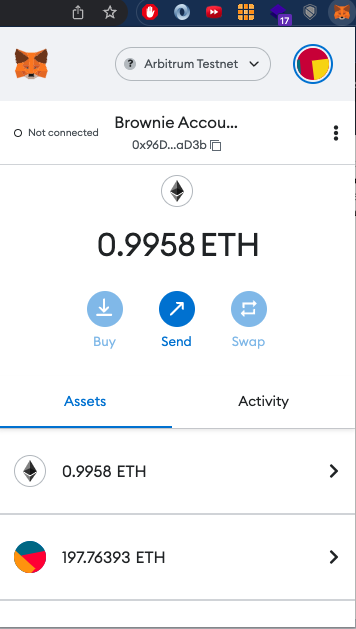
\includegraphics[scale=0.6]{metamask.png}
  \centering
  \caption{Screenshot di uno dei miei personali wallet su Metamask, estensione browser}
  \label{fig:metamask}
\end{figure}
\noindent \\WalletConnect è invece un protocollo che permette di integrare all'interno della propria dApp più tipologie di wallet (tra i quali anche Metamask).\\Le principali caratteristiche di WalletConnect sono \textbf{adattabilità} e \textbf{facilità di integrazione} con un qualsiasi portafoglio digitale: basterà che l'utente selezioni la propria wallet app o che inquadri un QR Code per effettuare immediatamente la connessione alla dApp di Orbit. 
\\\\Inoltre, è una valida soluzione per facilitare la connessione ad una dApp da dispositivi mobili, che allo stato attuale risulta ostica per la maggior parte dei prodotti Web3.

\subsection{Usabilità del sistema}

Nei mesi precedenti al lancio del prodotto, è stato svolto un importante lavoro di analisi di usabilità per rendere Orbit una piattaforma quanto più accessibile per i propri utenti, svolgendo delle sessione di \textbf{Beta Testing}, attraverso le quali sono sorti dubbi e feedback che hanno estremamente semplificato il flusso utente del prodotto finale. 
\\\\In quest'ultima parte, sono riuscito a dare il mio contributo attraverso nozioni imparate nel mio percorso di studi, in particolare in \textit{Interazione Uomo-Macchina}, quali principi di design dell'usabilità, scelta di palette cromatiche inclusive per persone con anomalie visive quali il daltonismo ed euristiche per facilitare l'esperienza utente.  

\section{Tecnologie Backend}

\subsection{Solidity}

\subsection{Hardhat}




\chapter{Architettura degli Smart Contracts di Orbit}


\chapter{Future implementazione all'interno di Orbit}


\bibliographystyle{unsrtnat}
\bibliography{bibliografia}




\end{document}